\documentclass[a4paper,12pt]{article}

\usepackage[T2A]{fontenc}
\usepackage[utf8]{inputenc}
\usepackage[english,russian]{babel}
\usepackage{indentfirst}
\usepackage{graphicx}
\usepackage{amsmath}
\usepackage{wrapfig}


\usepackage{caption}
\captionsetup{labelsep=period}


\begin{document}

\section*{\S 2.}

Пусть Рис. \ref{fg:21} представляет положение Солнца $S$, Земли $T$ и Луны $L$, и пусть центр $\Theta$ есть центр тяжести Земли и Луны. Делаем следующие обозначения:

\begin{table}[bhtp]
	\caption{}
	\begin{center}
	\begin{tabular}{|c|c|}
		\hline 
		Масса Солнца & $S$ \\ 
		\hline 
		Масса Земли & $T$ \\ 
		\hline 
		Масса Луны & $L$ \\ 
		\hline 
	\end{tabular} 
\end{center}
\end{table}

Расстояние:

\[
S \Theta = \phi; S T = \phi_1; S L = \phi_2; TL = r
\]

тогда будет:

\begin{equation}
\label{eq:1}
\begin{split}
T \Phi = r_1 = \frac{L}{T+L} \cdot r\\
L \Phi = r_2 = \frac{T}{T+L} \cdot r
\end{split}
\end{equation}

Составим теперь выражения ускорений, которые эти тела сообщают друг другу.

\begin{wrapfigure}{l}{0.4\linewidth}
	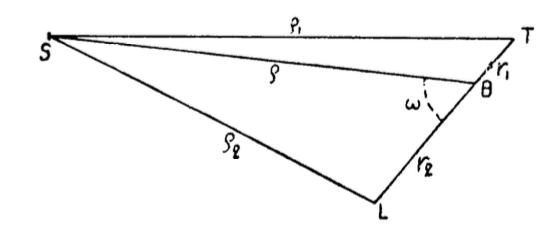
\includegraphics[width=\linewidth]{21.png}
	\caption{}
	\label{fg:21}
\end{wrapfigure}

Солнце $S$ сообщает ускорение:

\begin{center}
	Земле: $f \cdot \frac{S}{\rho_1^2}$ по направлению $TS$ \\
	Луне: $f \cdot \frac{S}{\rho_2^2}$ по направлению $LS$
\end{center}

вследствие чего тока $\Theta$ имеет ускорения:
\begin{center}
	$\frac{T}{T+L} \cdot f \cdot 	\frac{S}{\rho_1^2}$ по направлению, параллельному $TS$ \\
	$\frac{L}{T+L} \cdot f \cdot 	\frac{S}{\rho_2^2}$ по направлению, параллельному $LS$
\end{center}

Ускорения Солнца, происходящие от притяжения Земли и Луны, соответственно, суть:

\begin{center}
$f \cdot \frac{T}{\rho_1^2}$ по направлению $ST$ \\
$f \cdot \frac{L}{\rho_2^2}$ по направлению $SL$ \\
\end{center}

поэтому ускорения точки $\Theta$ относительно точки $S$ будут:
\begin{center}
	$w_1=f \cdot \frac{(S+T+L)}{T+L} \cdot \frac{T}{\rho_1^2}$ по направлению параллельно $TS$ \\
	$w_2=f \cdot \frac{(S+T+L)}{T+L} \cdot \frac{L}{\rho_2^2}$ по направлению параллельно $TL$ 
\end{center}

Разлагая эти ускорения, соответственно, по направлениям $\Theta S$ и $\Theta L$, получим, как легко видеть из подобия показанных на рис. \ref{fg:22} и рис. \ref{fg:23} треугольников:

\begin{center}
$w_1'=w_1 \cdot \frac{\rho}{\rho_1}$ \\
$w_1''=w_1 \cdot \frac{r_1}{\rho_1}$\\
$w_2'=w_2 \cdot \frac{\rho}{\rho_2}$\\
$w_1''=w_1 \cdot \frac{r_2}{\rho_2}$\\
\end{center}

\begin{figure}[bhtp]
	\caption{}
	\label{fg:22}
	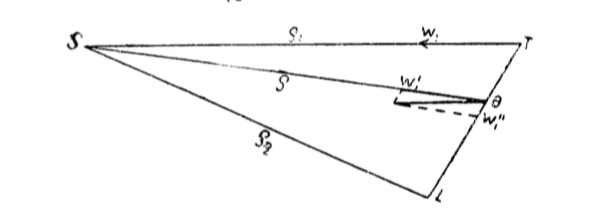
\includegraphics{22.png}
\end{figure}

получим для ускорения точки $\Theta$ слагающие:

\begin{center}
	$W_1 = w_1'+w_2'=f \cdot \frac{S+T+L}{T+L} \cdot \left[ T \cdot \frac{\rho}{\rho_1^3}+L \cdot \frac{\rho}{\rho_2^3}\right]$ по $\Theta S$ \\
	$W_2 = w_1''-w_2''=f \cdot \frac{S+T+L}{T+L} \cdot \left[ T \cdot \frac{r_1}{\rho_1^3}-L \cdot \frac{r_2}{\rho_2^3}\right]$ по $\Theta L$
\end{center}

\begin{figure}[bhtp]
	\caption{}
	\label{fg:23}
	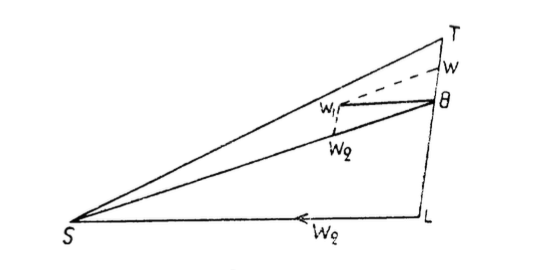
\includegraphics{23.png}
\end{figure}

Заменив $r_1$ и $r_2$ из выражения \eqref{eq:1}, имеем:
\begin{center}
	$W_1 = f \cdot \frac{S+T+L}{T+L} \cdot \rho \cdot \left[ \frac{T}{\rho_1^3}+\frac{L}{\rho_2^3} \right]$ по направлению $\Theta S$ \\
	$W_2 = f \cdot \frac{S+T+L}{T+L} \cdot T \cdot L \cdot r \cdot \left[ \frac{1}{\rho_1^3}-\frac{1}{\rho_2^3} \right]$ по направлению $\Theta L$
\end{center}

Но

\begin{center}
	$\rho_1^2 = \rho^2 + 2 \rho \cdot \frac{L}{T+L}\cdot r \cos\omega+\left(\frac{L}{T+L}\cdot r \right)^2$ \\
		$\rho_2^2 = \rho^2 - 2 \rho \cdot \frac{T}{T+L}\cdot r \cos\omega+\left(\frac{T}{T+L}\cdot r \right)^2$
\end{center}
следовательно

\begin{center}
$\frac{1}{\rho_1^3}=\frac{1}{\rho^3} \left[ 1+3\frac{L}{T+L}\cos \omega+\left( \frac{L}{T+L} \cdot r\right)^2 \left(-\frac{3}{2}+\frac{15}{2}\cos\omega^2 \right) + \ldots \right]$ \\
$\frac{1}{\rho_2^3}=\frac{1}{\rho^3} \left[ 1+3\frac{T}{T+L}\cos \omega+\left( \frac{L}{T+L} \cdot r\right)^2 \left(-\frac{3}{2}+\frac{15}{2}\cos\omega^2 \right) + \ldots \right]$ 
\end{center}
Подставляя эти выражения, имеем:

\begin{center}
	$W_1 = f \cdot \frac{S+T+L}{\rho^2} \cdot \left[ 1+ \frac{T \cdot L}{(T+L)^2} \cdot \frac{r^2}{\rho^2}\left(-\frac{3}{2}+\frac{15}{2}\cos\omega^2 \right) + \ldots \right]$\\
	$W_2 = f \cdot \frac{S+T+L}{\rho^2} \cdot \left[ -3 \cdot \frac{T \cdot L}{(T+L)^2} \cdot \frac{r^2}{\rho^2} \cos \omega + \ldots \right]$
\end{center}

Но отношения 
\begin{center}
	$\frac{L}{T+L} \approx \frac{1}{80}$; $\frac{r}{\rho} \approx \frac{1}{400}$; $\left(\frac{r}{\rho} \right)^2=\frac{1}{160000}$
\end{center}
поэтому будет

\begin{center}
	$\frac{T \cdot L}{(T+L)^2}\cdot \frac{r^2}{\rho^2} \approx \frac{1}{12800000}$
\end{center}

и члены, содержащие этот множитель, могут быть отброшены, так что будет:
\begin{center}
	$W_1=f \cdot \frac{S+T+L}{\rho^2}$ по направлению $\Theta S$ \\
	$W_2 = 0$ по направлению $\Theta L$
\end{center}

Отсюда следует, что точка $\Theta$ движется вокруг Солнца по эллептической орбите по законам Кеплера.

Рассмотрим теперь ускорение Луны по отнощению к Земле, для чего к ускорениям, сообщаемым Луне Солнцем и Землею, надо присовокупить ускорение, равное и противоположное ускорению Земли, происходящему от действия Солнца и Луны. Поступив подобно предыдущему, получим:

\begin{center}
	$f \cdot \frac{T+L}{r^2}+f\cdot S \left[ \frac{r_2}{\rho_2^3} +\frac{r_1}{\rho_1^3}\right]$ по направлению $L\Theta$ \\
	$f \cdot S \cdot \rho \left[\frac{1}{\rho_2^3}-\frac{1}{\rho_1^3} \right]$ параллельно $\Theta S$
\end{center}

положим:

\begin{center}
	$T+L= \mu$; $S=M$
\end{center}



\listoffigures
\listoftables
\end{document}